
\section{Тренинг}

Вася нарисовал схему и разработал плату замечательного устройсва --- фильтра
низкой частоты первого порядка. Плата была успешно изготовлена, спаяна и
настроена. Теперь это устройство безукоризненно выполняет свои функции на радость
клиентам фирмы, где работает Вася. Да вот беда --- начальство Васи требует
оформить перечень элементов согласно ЕСКД. Немного подумав, Вася решает
использовать для этих целей \emph{pcbdoc}.

Вася открывает свой любимый текстовый редактор(кто знает, возможно это
\emph{emacs}) и приступает к работе. Он аккуратно набирает первую строчку:

%\begin{SaveVerbatim}[formatcom=\bfseries]{TutorCode}
%\documentclass[doctype=pe]{pcbdoc}
%\end{SaveVerbatim}
%\colorbox{codecolor}{\BUseVerbatim{TutorCode}}

%\begin{tikzpicture}\node[align=left,fill=codecolor,font=\ttfamily] at (0,0){%
%\textbackslash{}documentclass[doctype=pe]\{pcbdoc\}
%};
%\end{tikzpicture}

\pcbdocmanualcode{%
\textbackslash{}documentclass[doctype=pe]\{pcbdoc\}
}

Теперь \LaTeX{} в курсе, что ему предстоит сверстать перечень элементов.
Далее Васе требуется указать, что он является автором этого замечательного
документа:

\begin{SaveVerbatim}{TutorCode}
  \AuthorSet{Пупкин}
\end{SaveVerbatim}
\colorbox{codecolor}{\BUseVerbatim{TutorCode}}

Готовый перечень элементов Вася планирует показать для проверки коллеге, который,
как и Вася, разрабатывает замечательные электронные устройства, рабочее место
которого находится неподалёку. Ну в самом деле, а вдруг в документ закрадётся
ошибка? Одна голова хорошо, а две лучше, думает Вася, набирая следующую
строчку:

\begin{SaveVerbatim}{TutorCode}
  \CheckerSet{Ближайший}
\end{SaveVerbatim}
\colorbox{codecolor}{\BUseVerbatim{TutorCode}}

Вася знает, что проверять готовый документ также будет и очень суровый
нормоконтролёр. Нужно указать и этот факт. Быстро и решительно Вася набирает
очередную строчку:

\begin{SaveVerbatim}{TutorCode}
  \NormControllerSet{Суровый}
\end{SaveVerbatim}
\colorbox{codecolor}{\BUseVerbatim{TutorCode}}

Вася знает, что утверждать перечень элементов будет Васин начальник. Вася очень
любит своего начальника, потому что он обещал повысить Васе зарплату. Жизнь
прекрасна, думает Вася, набирая следующую строчку:

\begin{SaveVerbatim}{TutorCode}
  \ApproverSet{Сказочник}
\end{SaveVerbatim}
\colorbox{codecolor}{\BUseVerbatim{TutorCode}}

Далее Вася указывает имя своего устройства и его децимальный номер, который
по секрету сообщил Васе его начальник отдела:

\begin{SaveVerbatim}{TutorCode}
  \NameSet{Фильтр}
  \NumberSet{РОГА.123456.001}
\end{SaveVerbatim}
\colorbox{codecolor}{\BUseVerbatim{TutorCode}}

Пора приступать к заполнению тела документа, думает Вася, набирая следующие
две строчки:

\begin{SaveVerbatim}{TutorCode}
  \begin{document}
  \begin{ElementList}
\end{SaveVerbatim}
\colorbox{codecolor}{\BUseVerbatim{TutorCode}}

Несмотря на то, что конденсатор в Васином устройстве всего один, Вася, вспомнив
про суровость нормоконтролёра,  решил создать для одного конденсатора целый
раздел:

\begin{SaveVerbatim}{TutorCode}
  \Part{Конденсаторы}
\end{SaveVerbatim}
\colorbox{codecolor}{\BUseVerbatim{TutorCode}}

Вот он, этот единственный конденсатор:

\begin{SaveVerbatim}{TutorCode}
  \Element{X7R\_0805\_1\_МКФ\_5\%}{\refbox{C1}}{1}
\end{SaveVerbatim}
\colorbox{codecolor}{\BUseVerbatim{TutorCode}}

Как видим, Вася не забыл указать его позиционное обозначение и
количество. Аналогично Вася поступил и с единственным резистором:

\begin{SaveVerbatim}{TutorCode}
  \Part{Резисторы}
  \Element{RMC\_0805\_1\_KOM\_5\%}{\refbox{R1}}{1}
\end{SaveVerbatim}
\colorbox{codecolor}{\BUseVerbatim{TutorCode}}

А вот соединителей в Васином устройстве целых два. Вася не забыл и про них:

\begin{SaveVerbatim}{TutorCode}
  \Part{Соединители}
  \Element{Розетка SMA-BJ}{\refbox{XS1,XS2}}{2}
\end{SaveVerbatim}
\colorbox{codecolor}{\BUseVerbatim{TutorCode}}

Ну вроде всё, подумал Вася. Пора закругляться.

\begin{SaveVerbatim}{TutorCode}
  \end{ElementList}
  \end{document}
\end{SaveVerbatim}
\colorbox{codecolor}{\BUseVerbatim{TutorCode}}

И сохранил полученный файл, присвоив ему имя \emph{vasia.tex}.

Открыв эмулятор терминала, Вася перешёл в директорию, куда он сохранил свой
файл, и скомпилировал его:

\begin{SaveVerbatim}{TutorCode}
  cd vasia
  xelatex vasia.tex
\end{SaveVerbatim}
\colorbox{terminalcolor}{\BUseVerbatim{TutorCode}}

После компиляции Вася обнаружил в своей рабочей директории файл
\emph{vasia.pdf}. Ну надо же, подумал Вася, получилось. Но что это за странные
вопросительные знаки в графе \emph{Листов}? Наверное, я что-то не то сделал,
подумал Вася, повторно запуская компиляцию:

\begin{SaveVerbatim}{TutorCode}
  xelatex vasia.tex
\end{SaveVerbatim}
\colorbox{terminalcolor}{\BUseVerbatim{TutorCode}}

После которой странные знаки исчезли. То-то же, подумал Вася и приступил к
настройке принтера. Распечатав полученный документ,

\begin{center}
\fcolorbox{black}{resultcolor}{%
%\begin{center}
  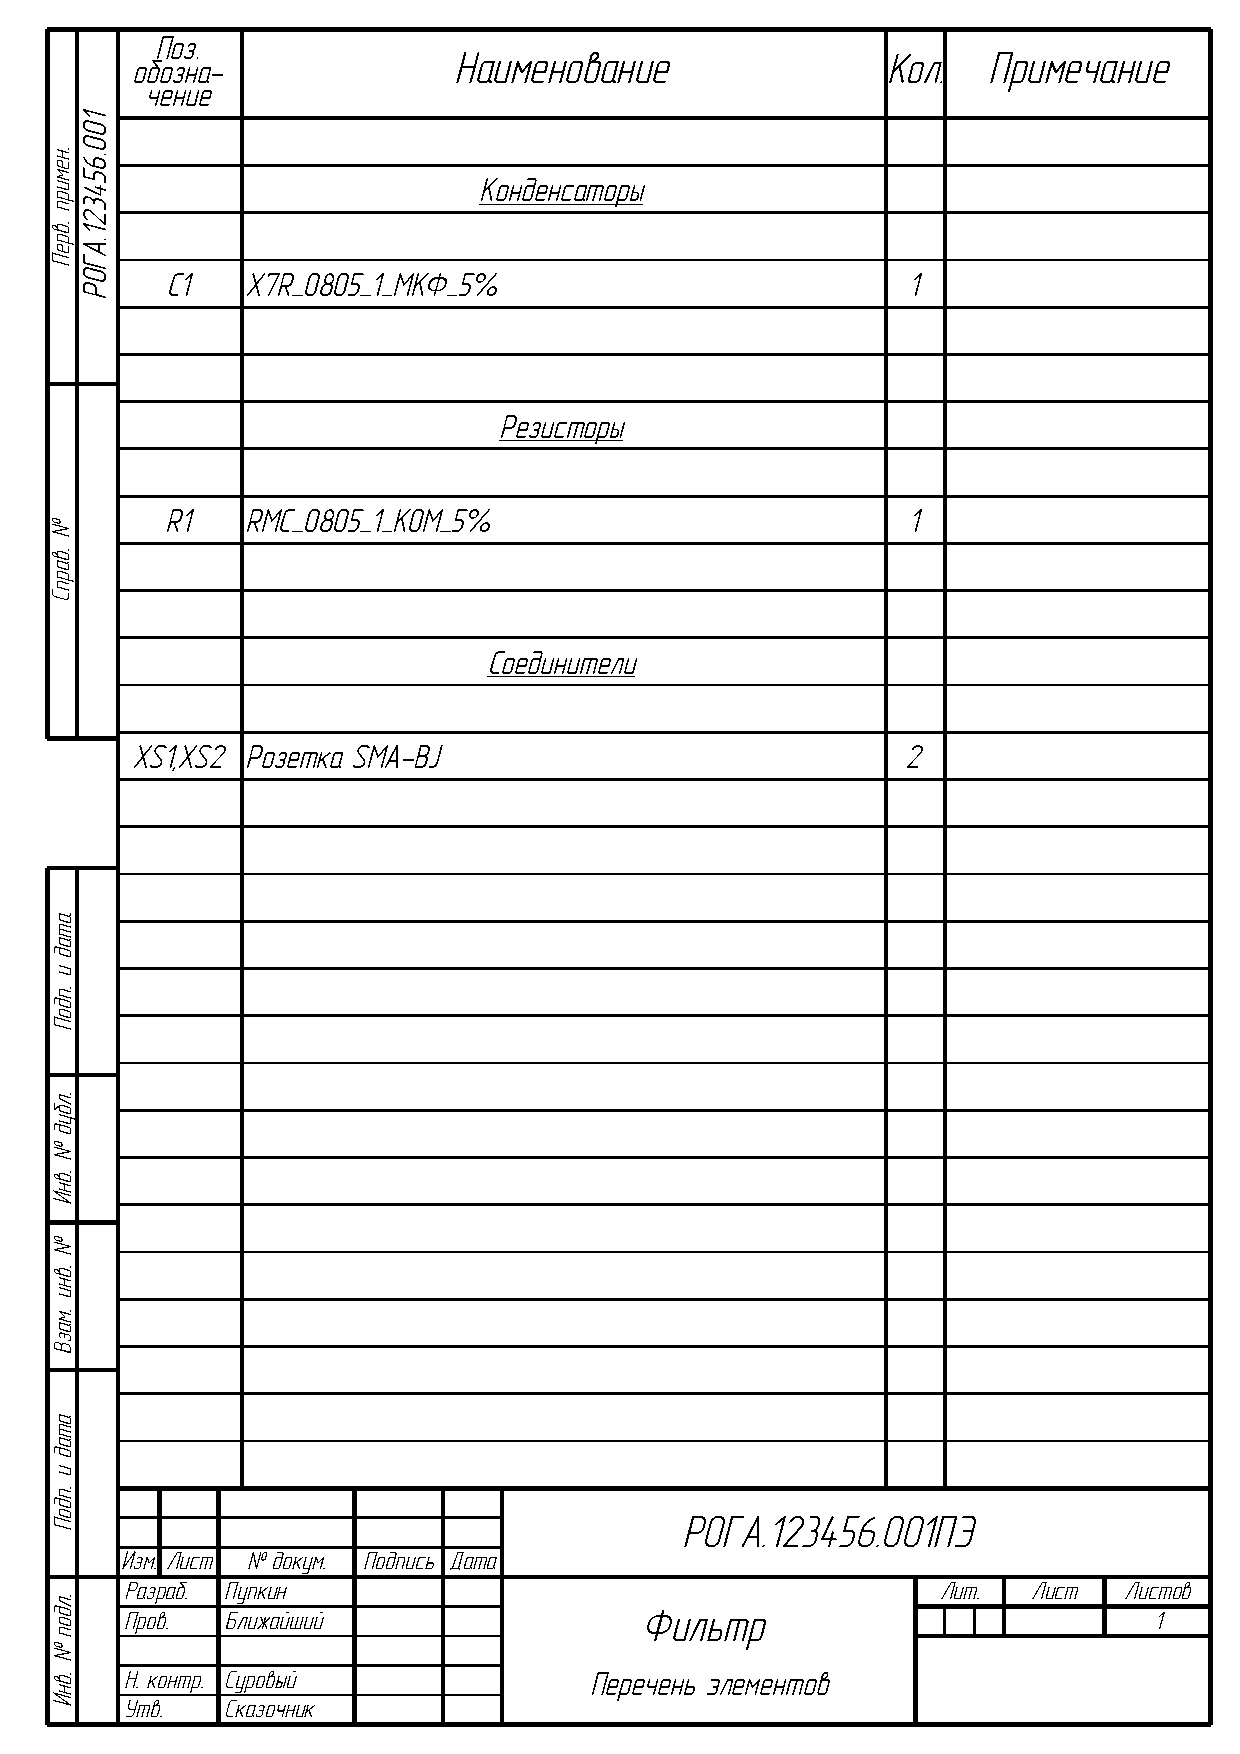
\includegraphics[scale=0.55]{output/vasia}
%\end{center}
}
\end{center}

Вася направился собирать подписи.
